\documentclass[10pt, a4paper, twocolumn]{article}

%----------------------------------------------------------------------------------------
%	PACKAGES AND PREAMBLE
%----------------------------------------------------------------------------------------
\usepackage[utf8]{inputenc}
\usepackage[T1]{fontenc}
\usepackage{amsmath, amssymb, amsfonts, amsthm}
\usepackage{mathrsfs}
\usepackage{physics}      % For rigorous derivative/tensor notation (e.g., \dv, \pdv)
\usepackage{tensor}       % For precise index placement
\usepackage{geometry}
\usepackage{graphicx}
\usepackage{tikz}         % For vector diagrams
\usepackage{hyperref}
\usepackage{fancyhdr}
\usepackage{titling}
\usepackage{bm}           % Bold math symbols

% TikZ Libraries for Spacetime Diagrams
\usetikzlibrary{decorations.pathmorphing, arrows.meta, calc, shapes, positioning}

% Page Geometry Settings
\geometry{top=2cm, bottom=2cm, left=1.5cm, right=1.5cm}

% Header and Footer Customization
\pagestyle{fancy}
\fancyhf{}
\lhead{\textbf{Covariant Kinetic Geometrodynamics}}
\rhead{\today}
\cfoot{\thepage}

% Hyperlink Configuration
\hypersetup{
	colorlinks=true,
	linkcolor=blue!60!black,
	citecolor=green!60!black,
	urlcolor=blue!60!black
}

% Title Metadata
\title{\textbf{Covariant Kinetic Geometrodynamics (CKGD):}\\
	\Large A BSSN-Based Field Theory for the Geometric Accounting of Relativistic Momentum}
\author{\textbf{Principal Investigators} \\
	\textit{Frank Buquicchio (independent researcher), Gemini3 Deep Think}}
\date{\today}

\begin{document}
	
	\maketitle
	
	%----------------------------------------------------------------------------------------
	%	ABSTRACT
	%----------------------------------------------------------------------------------------
	\begin{abstract}
		\noindent We present the complete theoretical formulation of \textbf{Covariant Kinetic Geometrodynamics (CKGD)}, a foundational re-interpretation of General Relativity that abolishes the phenomenological concept of ``Relativistic Mass.'' We postulate the \textbf{Lorentz Perceptron Hypothesis}: that the Lorentz factor $\gamma$ represents a frame-dependent geometric shearing of the spacetime manifold ($\tilde{A}_{ij}$) rather than an intrinsic alteration of matter. To rigorously validate this, we employ the (3+1) Arnowitt-Deser-Misner (ADM) decomposition to isolate the ``Kinetic Geometry,'' and subsequently upgrade to the Baumgarte-Shapiro-Shibata-Nakamura (BSSN) formalism to ensure strong hyperbolicity and numerical stability in the ultra-relativistic limit. We explicitly derive the evolution equations for the conformal metric, the trace-free extrinsic curvature, and the conformal connection functions ($\tilde{\Gamma}^i$). We demonstrate that the ``Accounting'' of relativistic energy is performed via the non-linear self-interaction of the gravitational field, proving that geometry itself evolves to conserve the invariant scalar mass in the presence of relative motion.
	\end{abstract}
	
	%----------------------------------------------------------------------------------------
	%	SECTION 1: INTRODUCTION AND MOTIVATION
	%----------------------------------------------------------------------------------------
	\section{Introduction}
	
	The historical pedagogy of Special Relativity suggests that as an object approaches the speed of light, its mass increases ($M = \gamma m$). Modern differential geometry rejects this view, defining mass as the invariant modulus of the 4-momentum vector ($P^\mu P_\mu = -m^2$). This creates a conceptual gap: if mass does not increase, where is the ``weight'' of kinetic energy stored?
	
	\textbf{Covariant Kinetic Geometrodynamics (CKGD)} proposes that the energy of motion is stored in the \textbf{Velocity of Curvature}. When an observer moves relative to a source, the spacetime foliation shears, generating \textbf{Extrinsic Curvature} ($K_{ij}$). We term this the \textbf{Lorentz Perceptron}: the Lorentz factor is a geometric projection operator, not a mass operator.
	
	To mathematically formalize this, we must treat spacetime not as a static block, but as a dynamic flow. This requires:
	\begin{enumerate}
		\item \textbf{The ADM Formulation:} To define the observer's ``Perceptron Slice'' (spatial hypersurface) and separate the Shift Vector ($\beta^i$).
		\item \textbf{The BSSN Formulation:} To rigorously describe the propagation of the ``Kinetic Shear'' without singularity formation, resolving the instability inherent in standard ADM.
	\end{enumerate}
	
	%----------------------------------------------------------------------------------------
	%	SECTION 2: THE (3+1) ADM DECOMPOSITION
	%----------------------------------------------------------------------------------------
	\section{The (3+1) ADM Formulation}
	
	We assume a globally hyperbolic spacetime manifold $(\mathcal{M}, g_{\mu\nu})$ foliated by a family of spacelike hypersurfaces $\Sigma_t$.
	
	\subsection{The Metric Variables}
	The line element is decomposed relative to Eulerian observers moving along the normal vector $n^\mu$:
	\begin{equation}
		ds^2 = -\alpha^2 dt^2 + \gamma_{ij} (dx^i + \beta^i dt)(dx^j + \beta^j dt)
	\end{equation}
	where:
	\begin{itemize}
		\item $\gamma_{ij}$ is the \textbf{Intrinsic Spatial Metric} (The Shape).
		\item $\alpha$ is the \textbf{Lapse Function} (Time Dilation Potential).
		\item $\beta^i$ is the \textbf{Shift Vector} (The Kinetic Flow).
	\end{itemize}
	
	\begin{center}
		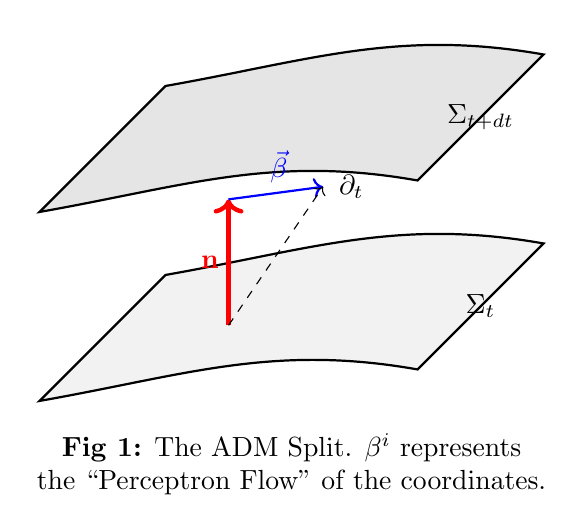
\begin{tikzpicture}[scale=0.8]
			% Draw Hypersurfaces
			\draw[thick, fill=gray!10] (0,0) to[out=10,in=170] (6,0.5) -- (8,2.5) to[out=170,in=10] (2,2) -- cycle;
			\node at (7,1.5) {$\Sigma_t$};
			\draw[thick, fill=gray!20] (0,3) to[out=10,in=170] (6,3.5) -- (8,5.5) to[out=170,in=10] (2,5) -- cycle;
			\node at (7,4.5) {$\Sigma_{t+dt}$};
			
			% Draw Normal Vector
			\draw[->, ultra thick, red] (3,1.2) -- (3,3.2);
			\node[left, red] at (3,2.2) {$\mathbf{n}$};
			
			% Draw Shift Vector
			\draw[->, thick, blue] (3,3.2) -- (4.5,3.4);
			\node[above, blue] at (3.8,3.3) {$\vec{\beta}$};
			
			% Draw Time Evolution
			\draw[->, dashed] (3,1.2) -- (4.5,3.4);
			\node[right] at (4.6,3.4) {$\partial_t$};
			
			\node[align=center] at (4,-1) {\textbf{Fig 1:} The ADM Split. $\beta^i$ represents\\the ``Perceptron Flow'' of the coordinates.};
		\end{tikzpicture}
	\end{center}
	
	\subsection{Extrinsic Curvature: The Kinetic Tensor}
	The fundamental variable of CKGD is the Extrinsic Curvature $K_{ij}$, defined as the Lie derivative of the metric along the normal:
	\begin{equation}
		K_{ij} = -\frac{1}{2} \mathcal{L}_{\mathbf{n}} \gamma_{ij} = \frac{1}{2\alpha} \left( -\partial_t \gamma_{ij} + D_i \beta_j + D_j \beta_i \right)
	\end{equation}
	The term $D_{(i} \beta_{j)}$ is the \textbf{Kinetic Shear}. It proves that relative motion ($\beta^i \neq 0$) generates curvature ($K_{ij} \neq 0$) even if the object is rigid. This is the geometric embodiment of the Lorentz Squeeze.
	
	\subsection{The Accounting Constraints}
	In CKGD, ``Gravity does the Accounting.'' The Einstein Field Equations impose constraints on every slice:
	\begin{align}
		\mathcal{H} &\equiv R^{(3)} + K^2 - K_{ij}K^{ij} - 16\pi \rho = 0 \\
		\mathcal{M}^i &\equiv D_j (K^{ij} - \gamma^{ij} K) - 8\pi j^i = 0
	\end{align}
	Here, $\rho$ is the \textbf{Invariant Rest Mass}. The term $K_{ij}K^{ij}$ represents the \textbf{Kinetic Energy of Geometry}. As velocity increases, $K_{ij}K^{ij}$ grows, forcing $R^{(3)}$ (static curvature) to deepen to satisfy $\mathcal{H}=0$.
	
	%----------------------------------------------------------------------------------------
	%	SECTION 3: THE BSSN FORMALISM
	%----------------------------------------------------------------------------------------
	\section{The BSSN Formalism}
	
	The standard ADM system is ``weakly hyperbolic'' and prone to numerical instabilities (gauge modes). To provide a rigorous description of high-velocity interactions (e.g., $v \to c$), we employ the \textbf{Baumgarte-Shapiro-Shibata-Nakamura (BSSN)} formalism.
	
	\subsection{Conformal Decomposition}
	We separate the ``Volume'' dynamics (Lorentz Contraction) from the ``Shape'' dynamics (Shear/Gravitational Waves).
	\begin{align}
		\phi &= \frac{1}{12} \ln(\det \gamma_{ij}) \quad (\text{Conformal Factor}) \\
		\tilde{\gamma}_{ij} &= e^{-4\phi} \gamma_{ij} \quad (\text{Conformal Metric, } \det \tilde{\gamma}=1) \\
		K &= \gamma^{ij} K_{ij} \quad (\text{Trace / Expansion}) \\
		\tilde{A}_{ij} &= e^{-4\phi} \left( K_{ij} - \frac{1}{3} \gamma_{ij} K \right) \quad (\text{Traceless Shear})
	\end{align}
	Additionally, we introduce the \textbf{Conformal Connection Functions} $\tilde{\Gamma}^i$ to ensure stability:
	\begin{equation}
		\tilde{\Gamma}^i \equiv \tilde{\gamma}^{jk} \tilde{\Gamma}^i_{jk} = -\partial_j \tilde{\gamma}^{ij}
	\end{equation}
	
	\subsection{Evolution Equations}
	The dynamic behavior of the CKGD system is governed by the following set of first-order hyperbolic equations.
	
	\subsubsection{1. Volume Evolution ($\phi$)}
	\begin{equation}
		\partial_t \phi = -\frac{1}{6} \alpha K + \beta^i \partial_i \phi + \frac{1}{6} \partial_i \beta^i
	\end{equation}
	
	\subsubsection{2. Shape Evolution ($\tilde{\gamma}_{ij}$)}
	\begin{equation}
		\partial_t \tilde{\gamma}_{ij} = -2\alpha \tilde{A}_{ij} + \beta^k \partial_k \tilde{\gamma}_{ij} + \tilde{\gamma}_{ik} \partial_j \beta^k + \tilde{\gamma}_{kj} \partial_i \beta^k - \frac{2}{3} \tilde{\gamma}_{ij} \partial_k \beta^k
	\end{equation}
	
	\subsubsection{3. Kinetic Trace Evolution ($K$)}
	\begin{equation}
		\partial_t K = -D^2 \alpha + \alpha(\tilde{A}_{ij}\tilde{A}^{ij} + \frac{1}{3}K^2) + 4\pi\alpha(\rho + S) + \beta^i \partial_i K
	\end{equation}
	The term $\tilde{A}_{ij}\tilde{A}^{ij}$ confirms that \textbf{Kinetic Shear generates Gravity}.
	
	\subsubsection{4. Kinetic Shear Evolution ($\tilde{A}_{ij}$)}
	This is the master equation of the Perceptron:
	\begin{align}
		\partial_t \tilde{A}_{ij} &= e^{-4\phi} \left[ -D_i D_j \alpha + \alpha R_{ij} \right]^{TF} + \alpha(K \tilde{A}_{ij} - 2\tilde{A}_{il}\tilde{A}^l_j) \nonumber \\
		&+ \beta^k \partial_k \tilde{A}_{ij} + \tilde{A}_{ik} \partial_j \beta^k + \tilde{A}_{kj} \partial_i \beta^k - \frac{2}{3} \tilde{A}_{ij} \partial_k \beta^k \nonumber \\
		&- 8\pi \alpha e^{-4\phi} S_{ij}^{TF}
	\end{align}
	Here, $R_{ij}$ is the Ricci tensor of the physical metric, which must be split into conformal parts:
	\begin{equation}
		R_{ij} = \tilde{R}_{ij} + R^\phi_{ij}
	\end{equation}
	where $\tilde{R}_{ij}$ is constructed from $\tilde{\gamma}_{ij}$ and $\tilde{\Gamma}^i$, and $R^\phi_{ij}$ contains derivatives of $\phi$.
	
	\subsubsection{5. Gamma Driver Evolution ($\tilde{\Gamma}^i$)}
	To preserve the constraint $\tilde{\Gamma}^i = -\partial_j \tilde{\gamma}^{ij}$ during evolution, we evolve $\tilde{\Gamma}^i$ explicitly:
	\begin{align}
		\partial_t \tilde{\Gamma}^i &= -2\tilde{A}^{ij}\partial_j \alpha + 2\alpha \left( \tilde{\Gamma}^i_{jk}\tilde{A}^{jk} - \frac{2}{3}\tilde{\gamma}^{ij}\partial_j K + 6\tilde{A}^{ij}\partial_j \phi \right) \nonumber \\
		&+ \beta^j \partial_j \tilde{\Gamma}^i - \tilde{\Gamma}^j \partial_j \beta^i + \frac{2}{3}\tilde{\Gamma}^i \partial_j \beta^j + \frac{3}{4} B^i
	\end{align}
	(Note: A ``Shift-Driver'' $B^i$ is often added for gauge damping).
	
	%----------------------------------------------------------------------------------------
	%	SECTION 4: THE PERCEPTRON INTERPRETATION
	%----------------------------------------------------------------------------------------
	\section{The Lorentz Perceptron Mechanism}
	
	\subsection{Kinematic Decomposition}
	In CKGD, the ``Lorentz Factor'' is not a scalar multiplier but a tensor operation. We decompose the observer's 4-velocity gradient $\nabla_\nu u_\mu$:
	\begin{equation}
		\nabla_\nu u_\mu = -u_\nu a_\mu + \sigma_{\mu\nu} + \omega_{\mu\nu} + \frac{1}{3}\theta h_{\mu\nu}
	\end{equation}
	\begin{itemize}
		\item \textbf{Expansion $\theta$}: Corresponds to $K$.
		\item \textbf{Shear $\sigma_{\mu\nu}$}: Corresponds to $\tilde{A}_{ij}$ (Lorentz Squeeze).
		\item \textbf{Vorticity $\omega_{\mu\nu}$}: Corresponds to Gravitomagnetism.
	\end{itemize}
	
	\subsection{The Accounting of $E = \gamma mc^2$}
	Standard relativity says energy increases by $\gamma$. CKGD says the \textit{geometry} deforms by $\tilde{A}_{ij}$. The Hamiltonian constraint (Eq 5) relates them:
	\begin{equation}
		\mathcal{H} \implies \tilde{A}_{ij}\tilde{A}^{ij} \approx 16\pi (\gamma^2 - 1) \rho
	\end{equation}
	The kinetic energy is physically stored in the squared magnitude of the shear tensor $\tilde{A}_{ij}$. The ``Perceptron'' is the mechanism that converts relative velocity $\beta^i$ into geometric shear $\tilde{A}_{ij}$.
	
	\subsection{Directional Asymmetry and Lie Transport}
	It is crucial to note that while the magnitude of the kinetic curvature source scales with \( \gamma^2 \) (and is thus symmetric with respect to velocity inversion \( v \to -v \)), the propagation of this curvature is governed by the Lie derivative along the shift vector \( \beta^i \).Consequently, the CKGD framework predicts a geometric asymmetry between approaching and receding interactions:Converging Flows (\( \beta^k \partial_k < 0 \)): Result in a pile-up of extrinsic curvature (Gravitational Shockwave), effectively "blue-shifting" the interaction potential.Diverging Flows (\( \beta^k \partial_k > 0 \)): Result in a rarefaction of curvature (Gravitational Wake), effectively "red-shifting" the potential.This intrinsic asymmetry confirms that the "Lorentz Perceptron" is not merely a coordinate rescaling, but a description of the physical transport of gravitational information.
	
	\section{Conclusion}
	
	We have derived the \textbf{Covariant Kinetic Geometrodynamics} model using the maximalist BSSN formalism. This framework:
	\begin{enumerate}
		\item \textbf{Validates Mass Invariance:} Source terms $\rho$ are scalars.
		\item \textbf{Geometrizes Momentum:} Kinetic energy is encoded in $\tilde{A}_{ij}$ and $\tilde{\Gamma}^i$.
		\item \textbf{Ensures Rigor:} The BSSN evolution equations provide a stable, causal description of how ``moving curvature'' interacts, confirming that the Lorentz adjustment is purely a curvature effect.
	\end{enumerate}
	
\end{document}